\documentclass[12pt]{article} % use larger type; default would be 10pt

\usepackage{pgfplots}
\usetikzlibrary{calc}
\usetikzlibrary{arrows}
\usetikzlibrary{patterns}
\usetikzlibrary{calc,intersections,through,backgrounds}
\usetikzlibrary{decorations.pathreplacing}
        \newcommand\degree[0]{^{\circ}}
        \newcommand\abs[1]{\left|#1\right|}

\title{Play with TikZ}
\author{Just Us}
%\date{} % Activate to display a given date or no date (if empty),
         % otherwise the current date is printed 

\begin{document}
\maketitle

\section{10.2 Polar Graphs }






fig10-2-1

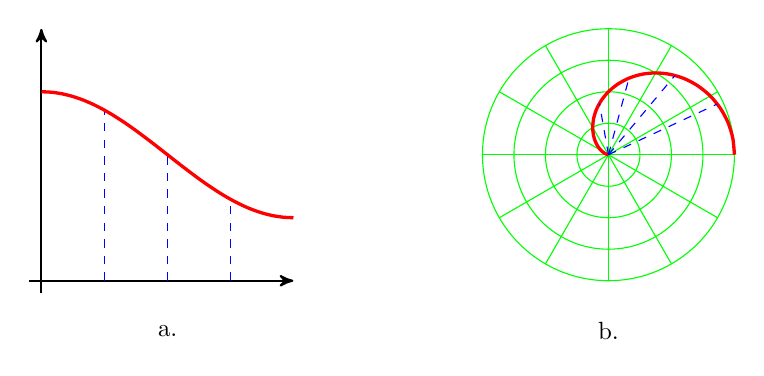
\begin{tikzpicture} [scale=1.6]
\def\d{-9/2};
\coordinate(O) at (\d,-1);
\draw[thick,->, >=stealth'] (O)++(-0.1,0) -- ($(O)+(2,0)$);
\draw[thick,->, >=stealth'] (O)++(0, -0.1) -- ($(O)+(0,2)$);
\foreach \x in {0.5, 1, 1.5} {
\draw[blue, dashed] (O)++(\x,0) -- ++($ (0,1)+0.5*cos(90*\x)*(0,1)$);
}
\draw[domain=0:2,smooth,variable=\x,red,very thick] plot ({\x+\d},{0.5*cos(90*\x))});
\node[text=black, scale=.9] at (-3.5,-1.4) {a.};


%polar 
\coordinate(O) at (0,0);
\foreach \angle [count=\xi] in {0, 30, ..., 330}{
  \draw[green] (\angle:0) -- (\angle:1);
}
\foreach \r in {0.25,.5,.75, 1}
\draw[green] (O) circle (\r);
\draw[domain=0:2,smooth,variable=\x,red,very thick] plot ({90*\x}:{0.5+0.5*cos(90*\x))});
\foreach \x in {0.25, 0.5, 0.75, 1} {
\draw[blue, dashed] (O) -- ({100*\x}:{0.5+0.5*cos(100*\x))});
}
\node[text=black, scale=.9] at (0,-1.4) {b.};

\end{tikzpicture}
\newline



exam10-2-1

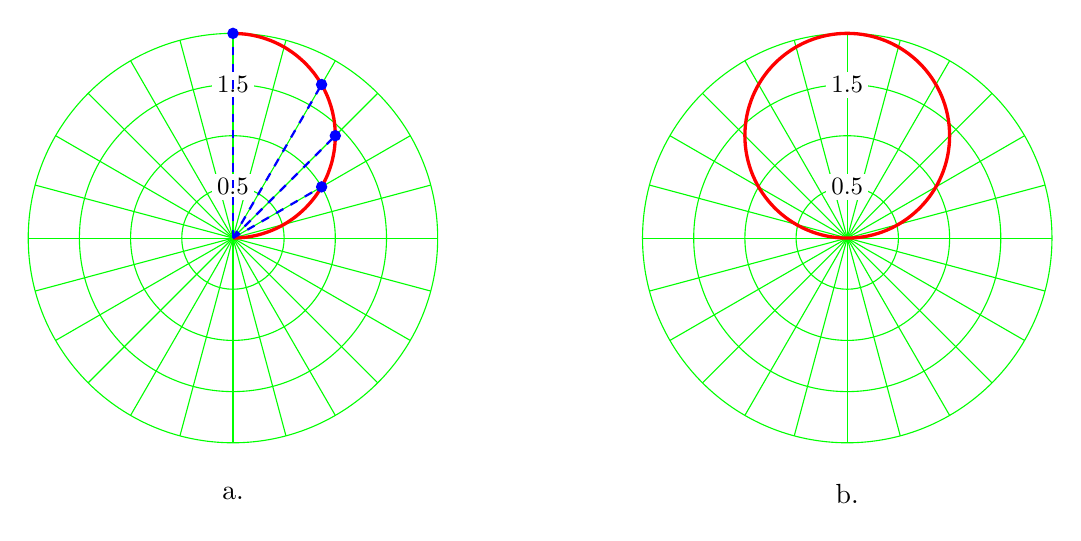
\begin{tikzpicture} [scale=1.3]
\coordinate(O) at (0,0);
\foreach \angle [count=\xi] in {0, 15, ..., 345}{
  \draw[green] (\angle:0) -- (\angle:2);
}
\foreach \r in {0.5,1,...,2} {
\draw[green] (O) circle (\r);
}
\foreach \r in {0.5,1.5} {
\node[fill=white, inner sep = 2, text=black, scale=.9] at (90:\r) {$\r$};
}
\draw[domain=0:3,smooth,variable=\x,red,very thick] plot ({30*\x}:{2*sin(30*\x))});
\foreach \x in {2,3,4,6} {
\draw[blue, thick, dashed] (O) -- ({15*\x}:{2*sin(15*\x))});
\filldraw[blue] ({15*\x}:{2*sin(15*\x))}) circle (0.05);
}

\node at (0,-2.5){a.};

%second grid
\coordinate(O) at (6,0);
\foreach \angle [count=\xi] in {0, 15, ..., 345}{
  \draw[green] (O)++(\angle:0) -- ++(\angle:2);
}
\foreach \r in {0.5,1,...,2} {
\draw[green] (O) circle (\r);
}
\foreach \r in {0.5,1.5} {
\node[fill=white, inner sep = 2, text=black, scale=.9] at ($(O)+(90:\r)$) {$\r$};
}
\draw[red,very thick] ($(O)+(0,1)$) circle (1cm) ;
\node at ($(O)+(0,-2.5)$){b.};

\end{tikzpicture}
\newline



exer10-2-1ans

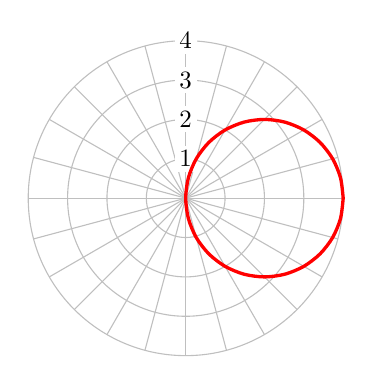
\begin{tikzpicture} [scale=0.5]
\coordinate(O) at (0,0);
\foreach \angle [count=\xi] in {0, 15, ..., 345}{
  \draw[lightgray] (\angle:0) -- (\angle:4);
}
\foreach \r in {1,2,3,4} {
\draw[lightgray] (O) circle (\r);
\node[fill=white, inner sep = 2, text=black, scale=.9] at (90:\r) {$\r$};
}
\draw[domain=0:6,smooth,variable=\x,red,very thick] plot ({30*\x}:{4*cos(30*\x))});

\end{tikzpicture}
\newline




exam10-2-2

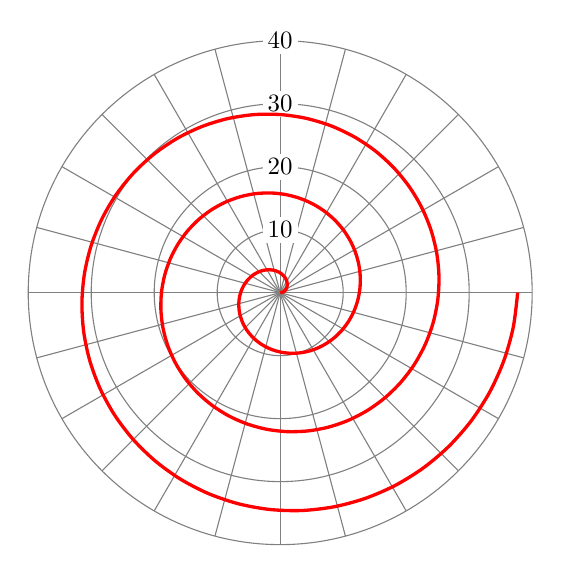
\begin{tikzpicture} [scale=0.08]
\coordinate(O) at (0,0);
\foreach \angle [count=\xi] in {0, 15, ..., 345}{
  \draw[gray] (\angle:0) -- (\angle:40);
}
\foreach \r in {10,20,30,40} {
\draw[gray] (O) circle (\r);
\node[fill=white, inner sep = 2, text=black, scale=.9] at (90:\r) {$\r$};
}
\draw[domain=0:3,smooth, samples=129,variable=\x,red,very thick] plot ({deg(2*pi*\x)}:{4*pi*\x});

\end{tikzpicture}
\newline




exer10-2-2ans

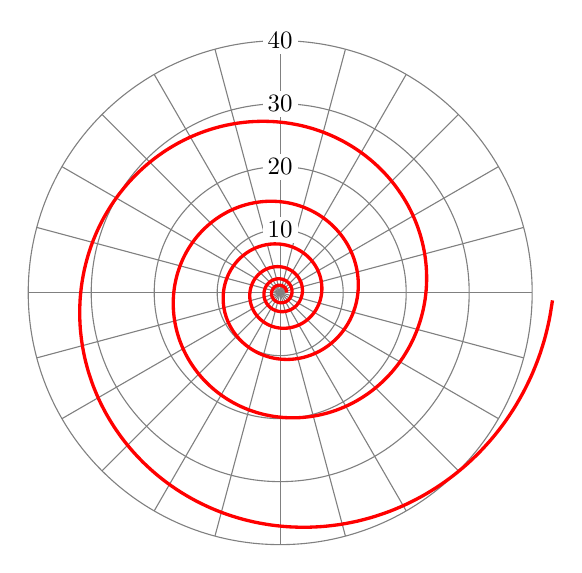
\begin{tikzpicture} [scale=0.08]
\coordinate(O) at (0,0);
\foreach \angle [count=\xi] in {0, 15, ..., 345}{
  \draw[gray] (\angle:0) -- (\angle:40);
}
\foreach \r in {10,20,30,40} {
\draw[gray] (O) circle (\r);
\node[fill=white, inner sep = 2, text=black, scale=.9] at (90:\r) {$\r$};
}
\draw[domain=0:6,smooth, samples=527,variable=\x,red,very thick] plot ({deg(2*pi*\x)}:{e^(0.2*pi*\x)});

\end{tikzpicture}
\newline



exam10-2-3a

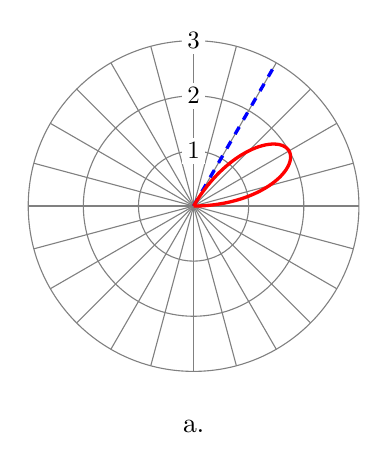
\begin{tikzpicture} [scale=0.7]
\coordinate(O) at (0,0);
\foreach \angle [count=\xi] in {0, 15, ..., 345}{
  \draw[gray] (\angle:0) -- (\angle:3);
}
\foreach \r in {1,2,3} {
\draw[gray] (O) circle (\r);
\node[fill=white, inner sep = 2, text=black, scale=.9] at (90:\r) {$\r$};
}
\draw[blue, very thick, dashed] (60:0) -- (60:3);
\draw[domain=0:4,smooth, samples=65,variable=\x,red,very thick] plot ({15*\x}:{2*sin(45*\x});
\node at (0,-4){a.};

\end{tikzpicture}
\newline



exam10-2-3b

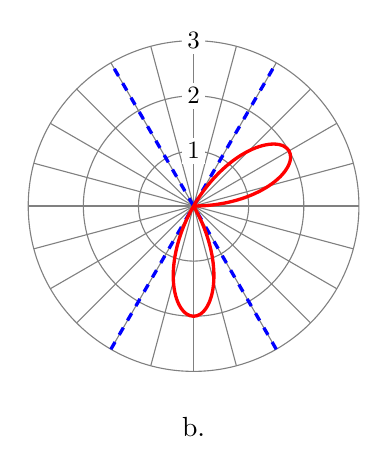
\begin{tikzpicture} [scale=0.7]
\coordinate(O) at (0,0);
\foreach \angle [count=\xi] in {0, 15, ..., 345}{
  \draw[gray] (\angle:0) -- (\angle:3);
}
\foreach \r in {1,2,3} {
\draw[gray] (O) circle (\r);
\node[fill=white, inner sep = 2, text=black, scale=.9] at (90:\r) {$\r$};
}
\draw[blue, very thick, dashed] (60:-3) -- (60:3);
\draw[blue, very thick, dashed] (120:-3) -- (120:3);
\draw[domain=0:8,smooth, samples=65,variable=\x,red,very thick] plot ({15*\x}:{2*sin(45*\x});
\node at (0,-4){b.};

\end{tikzpicture}
\newline



exam10-2-3c

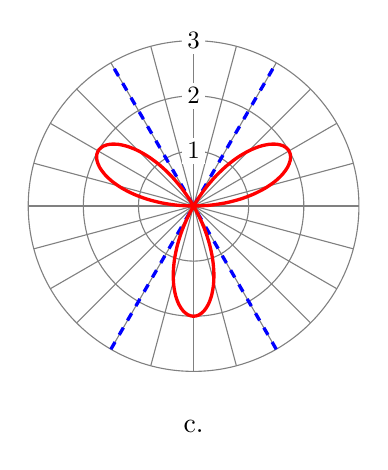
\begin{tikzpicture} [scale=0.7]
\coordinate(O) at (0,0);
\foreach \angle [count=\xi] in {0, 15, ..., 345}{
  \draw[gray] (\angle:0) -- (\angle:3);
}
\foreach \r in {1,2,3} {
\draw[gray] (O) circle (\r);
\node[fill=white, inner sep = 2, text=black, scale=.9] at (90:\r) {$\r$};
}
\draw[blue, very thick, dashed] (60:-3) -- (60:3);
\draw[blue, very thick, dashed] (120:-3) -- (120:3);
\draw[domain=0:12,smooth, samples=65,variable=\x,red,very thick] plot ({15*\x}:{2*sin(45*\x});
\node at (0,-4){c.};

\end{tikzpicture}
\newline

exer10-2-3 blank polar grid

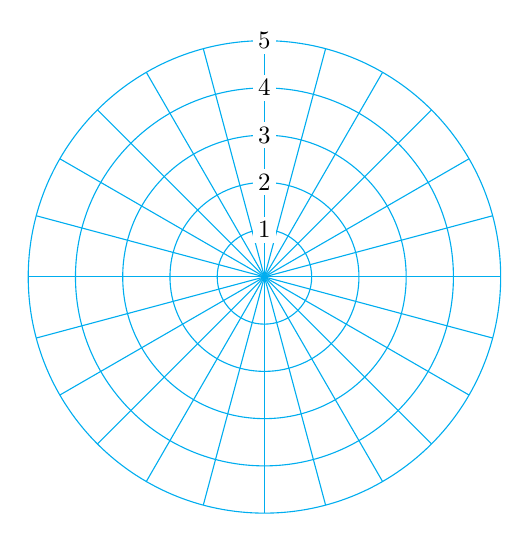
\begin{tikzpicture} [scale=.6]
\coordinate(O) at (0,0);
\foreach \angle [count=\xi] in {0, 15, ..., 345}{
  \draw[cyan] (\angle:0) -- (\angle:5);
}
\foreach \r in {1,2,3,4,5} {
\draw[cyan] (O) circle (\r);
\node[fill=white, inner sep = 2, text=black, scale=.9] at (90:\r) {$\r$};
}

\end{tikzpicture}
\newline

exer10-2-3ans three petal rose r = 2 cos(3 theta)

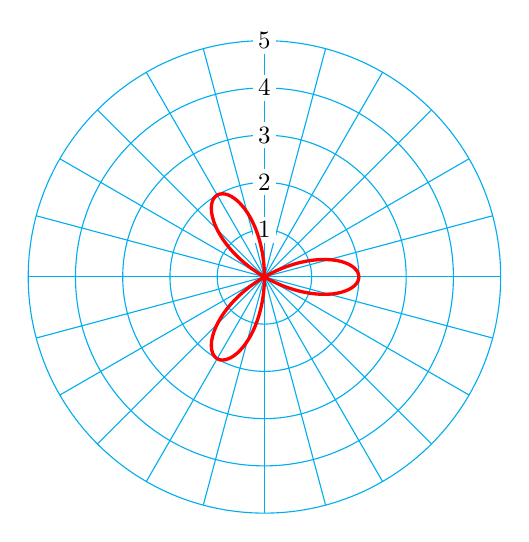
\begin{tikzpicture} [scale=.6]
\coordinate(O) at (0,0);
\foreach \angle [count=\xi] in {0, 15, ..., 345}{
  \draw[cyan] (\angle:0) -- (\angle:5);
}
\foreach \r in {1,2,3,4,5} {
\draw[cyan] (O) circle (\r);
\node[fill=white, inner sep = 2, text=black, scale=.9] at (90:\r) {$\r$};
}
\draw[domain=0:12,smooth, samples=65,variable=\x,red,very thick] plot ({15*\x}:{2*cos(45*\x});

\end{tikzpicture}
\newline


exam10-2-4 four petaled rose r = 3 sin (2 theta)

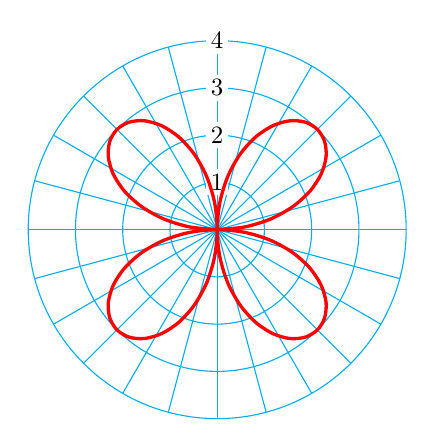
\begin{tikzpicture} [scale=.6]
\coordinate(O) at (0,0);
\foreach \angle [count=\xi] in {0, 15, ..., 345}{
  \draw[cyan] (\angle:0) -- (\angle:4);
}
\foreach \r in {1,2,3,4} {
\draw[cyan] (O) circle (\r);
\node[fill=white, inner sep = 2, text=black, scale=.9] at (90:\r) {$\r$};
}
\draw[domain=0:24,smooth, samples=65,variable=\x,red,very thick] plot ({15*\x}:{3*sin(30*\x});

\end{tikzpicture}
\newline


exer10-2-3ans five petaled rose r = 4 cos (5 theta)

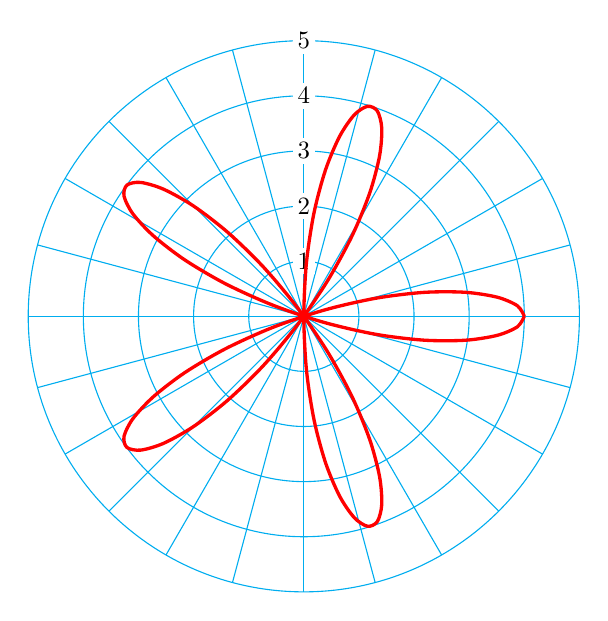
\begin{tikzpicture} [scale=.7]
\coordinate(O) at (0,0);
\foreach \angle [count=\xi] in {0, 15, ..., 345}{
  \draw[cyan] (\angle:0) -- (\angle:5);
}
\foreach \r in {1,2,3,4,5} {
\draw[cyan] (O) circle (\r);
\node[fill=white, inner sep = 2, text=black, scale=.9] at (90:\r) {$\r$};
}
\draw[domain=0:12,smooth, samples=65,variable=\x,red,very thick] plot ({15*\x}:{4*cos(75*\x});

\end{tikzpicture}
\newline


exam10-2-5 limacon r = 3 + 2 cos theta

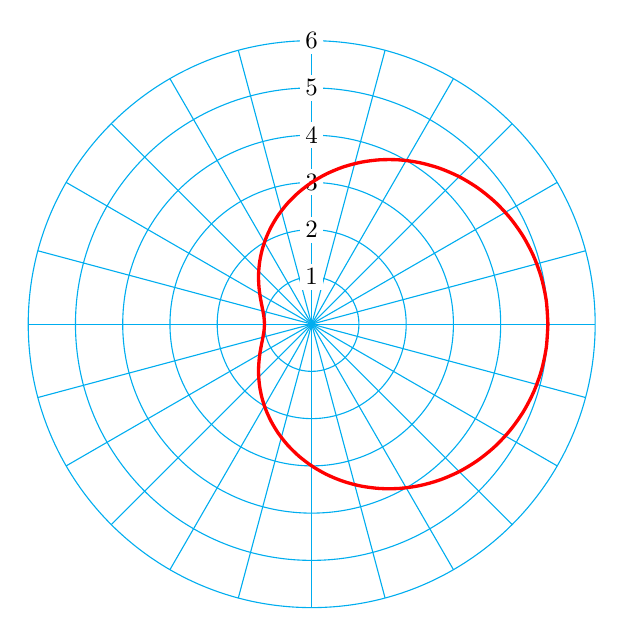
\begin{tikzpicture} [scale=.6]
\coordinate(O) at (0,0);
\foreach \angle [count=\xi] in {0, 15, ..., 345}{
  \draw[cyan] (\angle:0) -- (\angle:6);
}
\foreach \r in {1,2,3,4,5,6} {
\draw[cyan] (O) circle (\r);
\node[fill=white, inner sep = 2, text=black, scale=.9] at (90:\r) {$\r$};
}
\draw[domain=0:24,smooth, samples=65,variable=\x,red,very thick] plot ({15*\x}:{3+2*cos(15*\x});

\end{tikzpicture}
\newline


exer10-2-5ans limacon r = 1- 2 sin theta

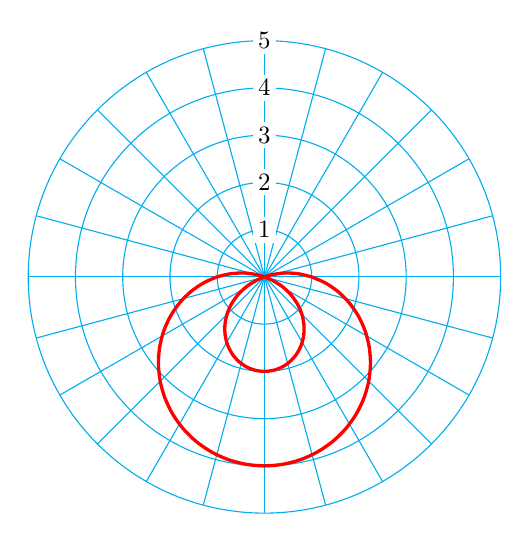
\begin{tikzpicture} [scale=.6]
\coordinate(O) at (0,0);
\foreach \angle [count=\xi] in {0, 15, ..., 345}{
  \draw[cyan] (\angle:0) -- (\angle:5);
}
\foreach \r in {1,2,3,4,5} {
\draw[cyan] (O) circle (\r);
\node[fill=white, inner sep = 2, text=black, scale=.9] at (90:\r) {$\r$};
}
\draw[domain=0:24,smooth, samples=65,variable=\x,red,very thick] plot ({15*\x}:{1-3*sin(15*\x});

\end{tikzpicture}
\newline



exam10-2-5a circle r = -4 cos theta

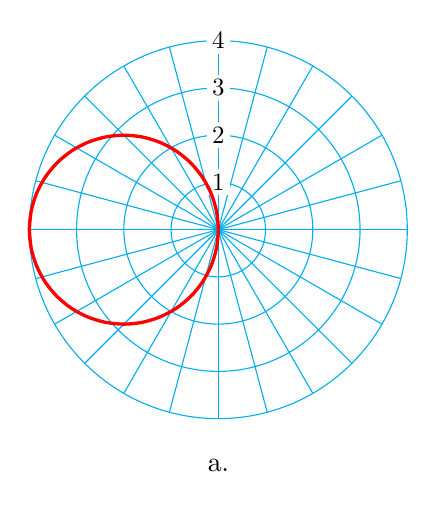
\begin{tikzpicture} [scale=.6]
\coordinate(O) at (0,0);
\foreach \angle [count=\xi] in {0, 15, ..., 345}{
  \draw[cyan] (\angle:0) -- (\angle:4);
}
\foreach \r in {1,2,3,4} {
\draw[cyan] (O) circle (\r);
\node[fill=white, inner sep = 2, text=black, scale=.9] at (90:\r) {$\r$};
}
\draw[domain=0:24,smooth, samples=65,variable=\x,red,very thick] plot ({15*\x}:{-4*cos(15*\x});
\node at (0,-5) {a.};

\end{tikzpicture}
\newline



exam10-2-5b cardioid r = 1 + cos theta

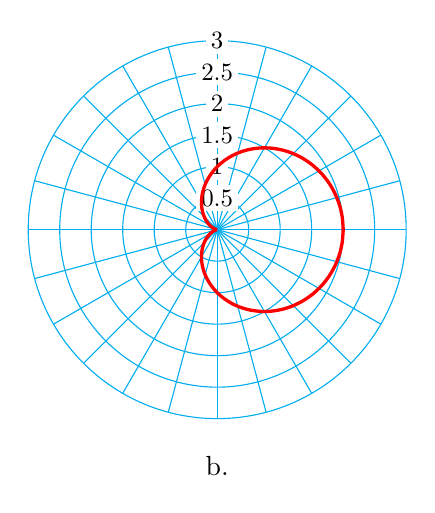
\begin{tikzpicture} [scale=.8]
\coordinate(O) at (0,0);
\foreach \angle [count=\xi] in {0, 15, ..., 345}{
  \draw[cyan] (\angle:0) -- (\angle:3);
}
\foreach \r in {0.5,1,1.5,2,2.5,3} {
\draw[cyan] (O) circle (\r);
\node[fill=white, inner sep = 2, text=black, scale=.9] at (90:\r) {$\r$};
}
\draw[domain=0:24,smooth, samples=65,variable=\x,red,very thick] plot ({15*\x}:{1+cos(15*\x});
\node at (0,-3.75) {b.};

\end{tikzpicture}
\newline



exer10-2-6a lemniscate r**2 = 4 sin theta

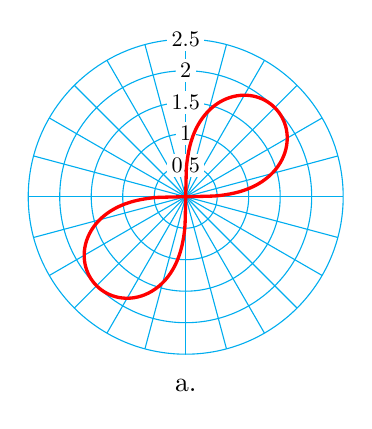
\begin{tikzpicture} [scale=.8]
\coordinate(O) at (0,0);
\foreach \angle [count=\xi] in {0, 15, ..., 345}{
  \draw[cyan] (\angle:0) -- (\angle:2.5);
}
\foreach \r in {0.5,1,1.5,2,2.5} {
\draw[cyan] (O) circle (\r);
\node[fill=white, inner sep = 2, text=black, scale=.8] at (90:\r) {$\r$};
}
\draw[domain=0:6,smooth, samples=65,variable=\x,red,very thick] plot ({15*\x}:{sqrt(4*sin(30*\x)});
\draw[domain=0:6,smooth, samples=65,variable=\x,red,very thick] plot ({15*\x}:{-sqrt(4*sin(30*\x)});
\node at (0,-3) {a.};

\end{tikzpicture}
\newline



exer10-2-6b cardioid r = 1- sin theta

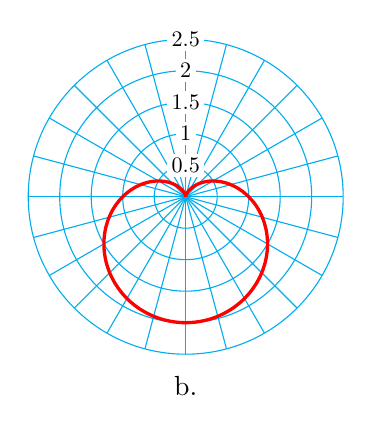
\begin{tikzpicture} [scale=.8]
\coordinate(O) at (0,0);
\foreach \angle [count=\xi] in {0, 15, ..., 345}{
  \draw[cyan] (\angle:0) -- (\angle:2.5);
}
\foreach \r in {0.5,1,1.5,2,2.5} {
\draw[cyan] (O) circle (\r);
\node[fill=white, inner sep = 2, text=black, scale=.8] at (90:\r) {$\r$};
}
\draw[domain=0:24,smooth, samples=65,variable=\x,red,very thick] plot ({15*\x}:{1-sin(15*\x});
\node at (0,-3) {b.};

\end{tikzpicture}
\newline



fig10-2-2 line intersecting parabola

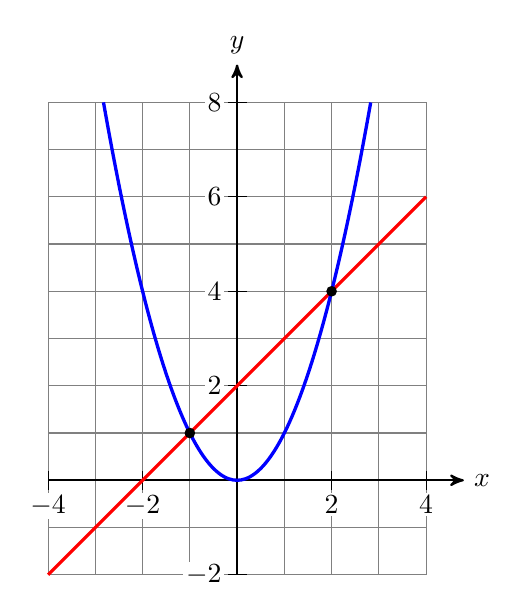
\begin{tikzpicture} [scale=.6]
\coordinate(O) at (0,0);
\draw[gray] (-4,-2) grid (4,8);
\draw[thick,black,->,>=stealth'] (-4,0)--(4.8,0) node[right]{$x$};
\draw[thick,black,->,>=stealth'] (0,-2)--(0,8.8) node[above]{$y$};
\foreach \x  in {2,4}{
  \draw[black] (\x, .2) -- ++(0,-.4) node[below, yshift=-1, fill=white, inner sep=1]{$\x$};
  \draw[black] (-\x, .2) -- ++(0,-.4) node[below, yshift=-1, fill=white, inner sep=1]{$-\x$};
}
\foreach \y  in {2,4,6,8}{
  \draw[black] (.2,\y) -- ++(-.4,0) node[left, xshift=-1, fill=white, inner sep=1]{$\y$};
}
\draw[black] (.2,-2) -- ++(-.4,0) node[left, xshift=-1, fill=white, inner sep=1]{$-2$};

\draw[red,very thick] (-4,-2)--(4,6);
\draw[domain=-sqrt(8):sqrt(8),smooth, samples=65,variable=\x,blue,very thick] plot (\x, {(\x)^2});
\filldraw[black] (2,4) circle (.1);
\filldraw[black] (-1,1) circle (.1);

\end{tikzpicture}
\newline


exam10-2-7 cardioids r = 2 + 2 sin theta and r = 2 + 2 cos theta

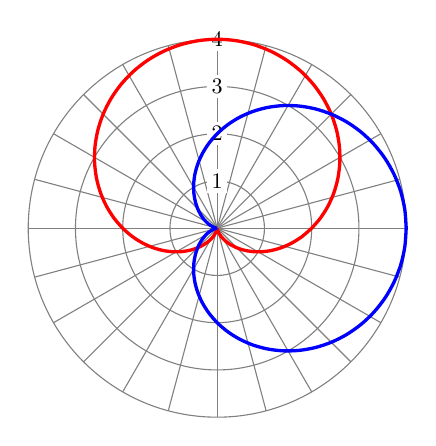
\begin{tikzpicture} [scale=.6]
\coordinate(O) at (0,0);
\foreach \angle [count=\xi] in {0, 15, ..., 345}{
  \draw[gray] (\angle:0) -- (\angle:4);
}
\foreach \r in {1,2,3,4} {
\draw[gray] (O) circle (\r);
\node[fill=white, inner sep = 2, text=black, scale=.8] at (90:\r) {$\r$};
}
\draw[domain=0:24,smooth, samples=65,variable=\x,red,very thick] plot ({15*\x}:{2+2*sin(15*\x});
\draw[domain=0:24,smooth, samples=65,variable=\x,blue,very thick] plot ({15*\x}:{2+2*cos(15*\x});

\end{tikzpicture}
\newline


cat10-2-1 line

\begin{tikzpicture} 
\draw[black, ->,>=stealth'] (-2,0)--(2,0);
\draw[gray] (0,-2)--(0,2);
\def\theta{65};
\draw[red,thick] (\theta:{2/sin(\theta)}) --({180+\theta}:{2/sin(\theta)});
\draw[lightgray, ->, >=stealth'] (.5,0) arc(0:\theta:0.5) node[above right, yshift=-4, midway, text=red] {$k$};

\end{tikzpicture}
\newline


cat10-2-2 circle

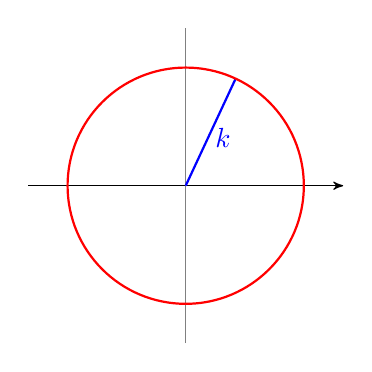
\begin{tikzpicture} 
\draw[black, ->,>=stealth'] (-2,0)--(2,0);
\draw[gray] (0,-2)--(0,2);
\def\k{1.5};
\draw[blue,thick] (0,0) --(65:\k) node[below right, xshift=-2, yshift=5, midway,text=blue] {$k$};
\draw[red, thick] (0,0) circle (\k);
\end{tikzpicture}
\newline



cat10-2-3 circle

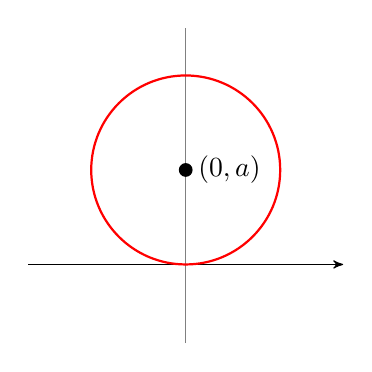
\begin{tikzpicture} 
\draw[black, ->,>=stealth'] (-2,0)--(2,0);
\draw[gray] (0,-1)--(0,3);
\draw[red, thick] (0,1.2) circle (1.2);
\filldraw[black] (0,1.2) circle (0.08) node[right, xshift=1] {$(0,a)$};
\end{tikzpicture}
\newline



cat10-2-4 circle

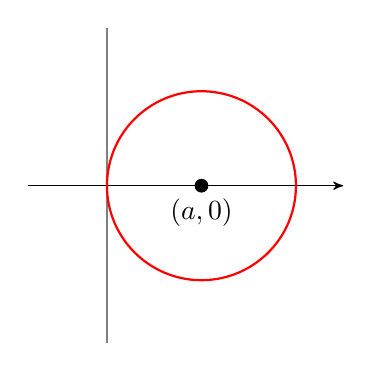
\begin{tikzpicture} 
\draw[black, ->,>=stealth'] (-1,0)--(3,0);
\draw[gray] (0,-2)--(0,2);
\draw[red, thick] (1.2,0) circle (1.2);
\filldraw[black] (1.2,0) circle (0.08) node[below, yshift=-1] {$(a,0)$};
\end{tikzpicture}
\newline


cat10-2-5 Rose a sin n theta

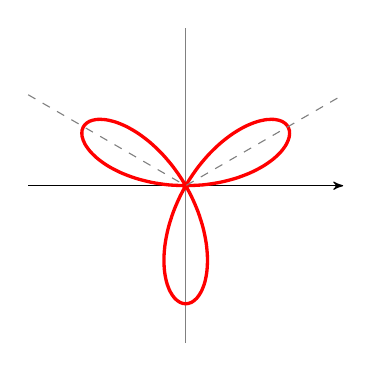
\begin{tikzpicture} 
\draw[black, ->,>=stealth'] (-2,0)--(2,0);
\draw[gray] (0,-2)--(0,2);
\draw[domain=0:12,smooth, samples=65,variable=\x,red,very thick] plot ({15*\x}:{1.5*sin(45*\x});
\draw[gray, dashed] (-2,{2/sqrt(3)})--(0,0)--(2,{2/sqrt(3)});
\end{tikzpicture}
\newline


cat10-2-6 Rose a cos n theta

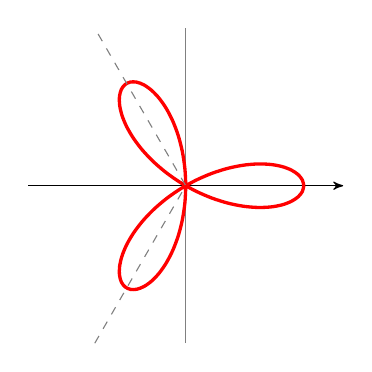
\begin{tikzpicture} 
\draw[black, ->,>=stealth'] (-2,0)--(2,0);
\draw[gray] (0,-2)--(0,2);
\draw[domain=0:12,smooth, samples=65,variable=\x,red,very thick] plot ({15*\x}:{1.5*cos(45*\x});
\draw[gray, dashed] ({-2/sqrt(3)}, -2)--(0,0)--({-2/sqrt(3)}, 2);
\end{tikzpicture}
\newline


cat10-2-7 limacon a + b cos theta, a larger

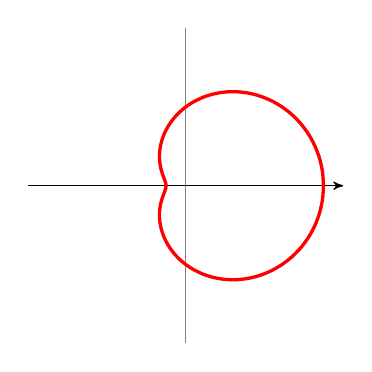
\begin{tikzpicture} 
\draw[black, ->,>=stealth'] (-2,0)--(2,0);
\draw[gray] (0,-2)--(0,2);
\draw[domain=0:24,smooth, samples=65,variable=\x,red,very thick] plot ({15*\x}:{1 + .75*cos(15*\x});
\end{tikzpicture}
\newline


cat10-2-8 limacon a + b sin theta, a smaller

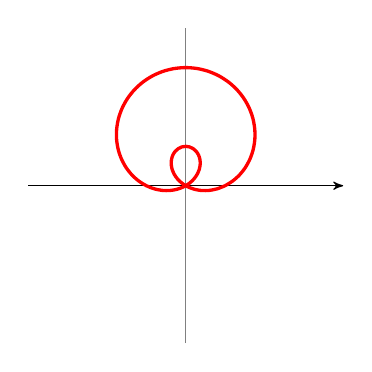
\begin{tikzpicture} 
\draw[black, ->,>=stealth'] (-2,0)--(2,0);
\draw[gray] (0,-2)--(0,2);
\draw[domain=0:24,smooth, samples=65,variable=\x,red,very thick] plot ({15*\x}:{.5 + 1*sin(15*\x});
\end{tikzpicture}
\newline


cat10-2-9 cardioid a + a sin theta

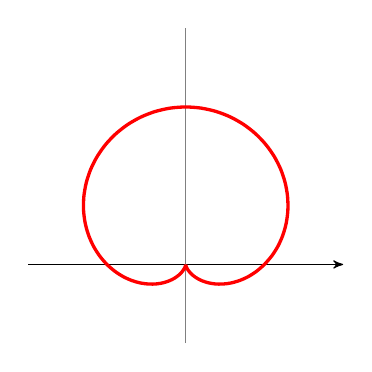
\begin{tikzpicture} 
\draw[black, ->,>=stealth'] (-2,0)--(2,0);
\draw[gray] (0,-1)--(0,3);
\draw[domain=0:24,smooth, samples=65,variable=\x,red,very thick] plot ({15*\x}:{1 + 1*sin(15*\x});
\end{tikzpicture}
\newline


cat10-2-10 lemniscape r**2 = a**2 cos 2 theta

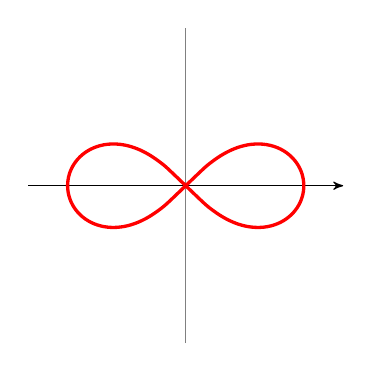
\begin{tikzpicture} 
\draw[black, ->,>=stealth'] (-2,0)--(2,0);
\draw[gray] (0,-2)--(0,2);
\draw[domain=-3:3,smooth, samples=65,variable=\x,red,very thick] plot ({15*\x}:{1.5*sqrt(cos(30*\x)});
\draw[domain=-3:3,smooth, samples=65,variable=\x,red,very thick] plot ({15*\x}:{-1.5*sqrt(cos(30*\x)});
\end{tikzpicture}
\newline


cat10-2-11 lemniscape r**2 = a**2 sin 2 theta

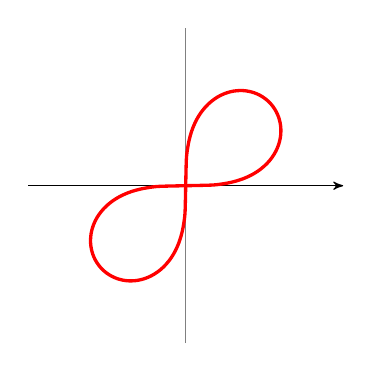
\begin{tikzpicture} 
\draw[black, ->,>=stealth'] (-2,0)--(2,0);
\draw[gray] (0,-2)--(0,2);
\draw[domain=0:6,smooth, samples=65,variable=\x,red,very thick] plot ({15*\x}:{1.5*sqrt(sin(30*\x)});
\draw[domain=0:6,smooth, samples=65,variable=\x,red,very thick] plot ({15*\x}:{-1.5*sqrt(sin(30*\x)});
\end{tikzpicture}
\newline


cat10-2-12 Archimedean spiral r = a theta

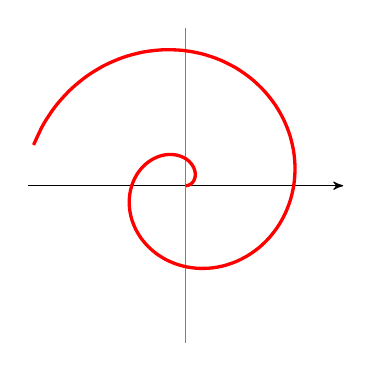
\begin{tikzpicture} 
\draw[black, ->,>=stealth'] (-2,0)--(2,0);
\draw[gray] (0,-2)--(0,2);
\draw[domain=0:35,smooth, samples=65,variable=\x,red,very thick] plot ({15*\x}:{\x/17.5});
\end{tikzpicture}
\newline


cat10-2-13 logarithmic spiral r = e**(a theta)

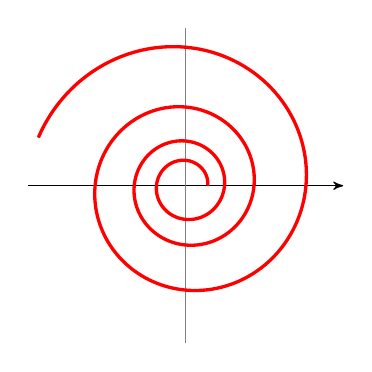
\begin{tikzpicture} 
\draw[black, ->,>=stealth'] (-2,0)--(2,0);
\draw[gray] (0,-2)--(0,2);
\draw[domain=0:3.45,smooth, samples=527,variable=\x,red,very thick] plot ({deg(2*pi*\x)}:{0.28*e^(0.18*pi*\x)});
\end{tikzpicture}
\newline


hp10-2-1ans circles

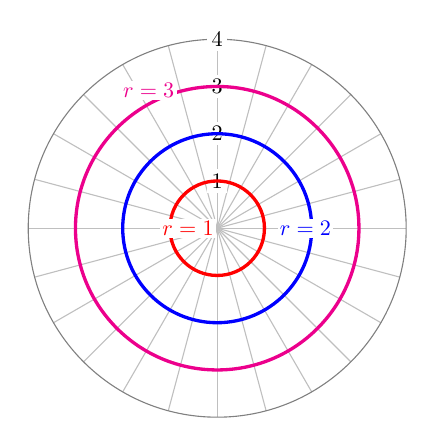
\begin{tikzpicture} [scale=.6]
\coordinate(O) at (0,0);
\foreach \angle [count=\xi] in {0, 15, ..., 345}{
  \draw[lightgray] (\angle:0) -- (\angle:4);
}
\foreach \r in {1,2,3,4} {
\draw[gray] (O) circle (\r);
\node[fill=white, inner sep = 2, text=black, scale=.8] at (90:\r) {$\r$};
}
\draw[red,very thick] (O) circle (1cm) node[left, fill=white, inner sep=1, scale=.8] {$r=1$};
\draw[blue,very thick] (O) circle (2cm) node[right, xshift=0.75cm, fill=white, inner sep=1, scale=.8] {$r=2$};
\draw[magenta,very thick] (O) circle (3cm) node[left, xshift=-.5cm, yshift=1.75cm, fill=white, inner sep=1, scale=.8] {$r=3$};
\end{tikzpicture}
\newline


hp10-2-3ans lines

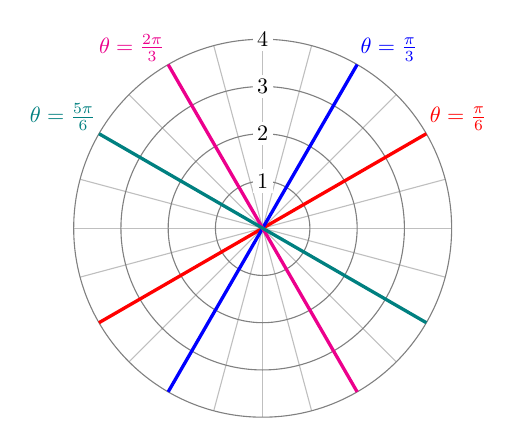
\begin{tikzpicture} [scale=.6]
\coordinate(O) at (0,0);
\foreach \angle [count=\xi] in {0, 15, ..., 345}{
  \draw[lightgray] (\angle:0) -- (\angle:4);
}
\foreach \r in {1,2,3,4} {
\draw[gray] (O) circle (\r);
\node[fill=white, inner sep = 2, text=black, scale=.8] at (90:\r) {$\r$};
}
\draw[red,very thick] (210:4)-- (30:4) node[above right, fill=white, inner sep=1, scale=.8] {$\theta=\frac{\pi}{6}$};
\draw[blue,very thick] (240:4) -- (60:4) node[above right, fill=white, inner sep=1, scale=.8] {$\theta=\frac{\pi}{3}$};
\draw[magenta,very thick] (300:4) -- (120:4) node[above left, fill=white, inner sep=1, scale=.8] {$\theta=\frac{2\pi}{3}$};
\draw[teal,very thick] (330:4) -- (150:4) node[above left, fill=white, inner sep=1, scale=.8] {$\theta=\frac{5\pi}{6}$};
\end{tikzpicture}
\newline


hp10-2-5ans points on circle

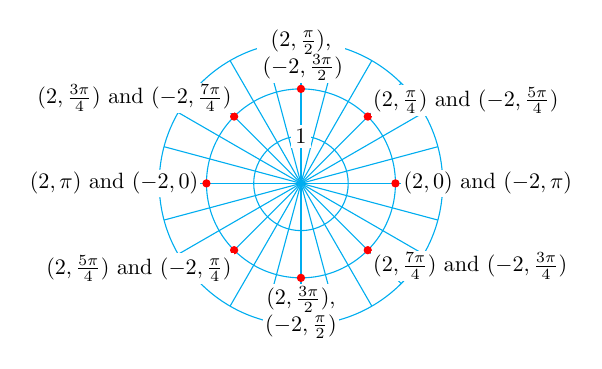
\begin{tikzpicture} [scale=.6]
\coordinate(O) at (0,0);
\foreach \angle [count=\xi] in {0, 15, ..., 345}{
  \draw[cyan] (\angle:0) -- (\angle:3);
}
\foreach \r in {1,2,3} {
\draw[cyan] (O) circle (\r);
}
\node[fill=white, inner sep = 2, text=black, scale=.8] at (90:1) {$1$};

\filldraw[red] (0:2)circle (.075) node[right, text=black, fill=white, inner sep=1, xshift=2, scale=.8] {$(2,0)$ and $(-2,\pi)$};
\filldraw[red] (45:2)circle (.075) node[above right, text=black, fill=white, inner sep=1, xshift=1, scale=.8] {$(2,\frac{\pi}{4})$ and $(-2,\frac{5\pi}{4})$};
\filldraw[red] (90:2)circle (.075) node[above,align=center, text=black, fill=white, inner sep=1, yshift=2, scale=.8] {$(2,\frac{\pi}{2})$, \\ $\,(-2,\frac{3\pi}{2})$};
\filldraw[red] (135:2)circle (.075) node[above left, text=black, fill=white, inner sep=1, yshift=1, scale=.8] {$(2,\frac{3\pi}{4})$ and $(-2,\frac{7\pi}{4})$};
\filldraw[red] (180:2)circle (.075) node[left, text=black, fill=white, inner sep=1, xshift=-2, scale=.8] {$(2,\pi)$ and $(-2,0)$};
\filldraw[red] (225:2)circle (.075) node[below left, text=black, fill=white, inner sep=1, yshift=-1, scale=.8] {$(2,\frac{5\pi}{4})$ and $(-2,\frac{\pi}{4})$};
\filldraw[red] (270:2)circle (.075) node[below,align=center, yshift=0cm, text=black, fill=white, inner sep=1, yshift=-2, scale=.8] {$(2,\frac{3\pi}{2})$, \\ $(-2,\frac{\pi}{2})$};
\filldraw[red] (315:2)circle (.075) node[below right, text=black, fill=white, inner sep=1, xshift=1, scale=.8] {$(2,\frac{7\pi}{4})$ and $(-2,\frac{3\pi}{4})$};
\end{tikzpicture}
\newline


hp10-2-7ans points on circle

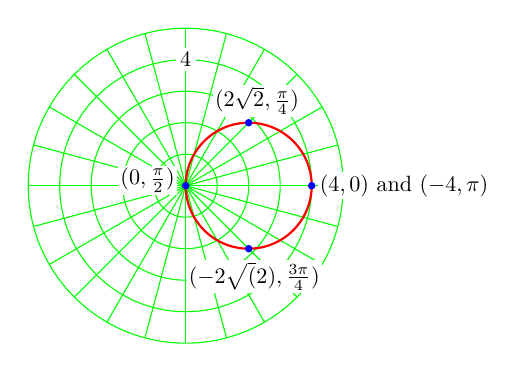
\begin{tikzpicture} [scale=.4]
\coordinate(O) at (0,0);
\foreach \angle [count=\xi] in {0, 15, ..., 345}{
  \draw[green] (\angle:0) -- (\angle:5);
}
\foreach \r in {1,2,3,4,5} {
\draw[green] (O) circle (\r);
}
\node[fill=white, inner sep = 2, text=black, scale=.8] at (90:4) {$4$};
\draw[red,thick] (2,0) circle (2cm);
\filldraw[blue] (0:4)circle (.1) node[right, text=black, fill=white, inner sep=1, xshift=2, scale=.8] {$(4,0)$ and $(-4,\pi)$};
\filldraw[blue] (45:{2*sqrt(2)})circle (.1) node[above, xshift=2, yshift=2, text=black, fill=white, inner sep=1, xshift=1, scale=.8] {$(2\sqrt{2},\frac{\pi}{4})$};
\filldraw[blue] (90:0)circle (.1) node[left, xshift=-3, text=black, fill=white, inner sep=1, yshift=2, scale=.8] {$(0,\frac{\pi}{2})$};
\filldraw[blue] (315:{2*sqrt(2)})circle (.1) node[below, text=black, fill=white, inner sep=1, xshift=2, yshift=-4, scale=.8] {$(-2\sqrt(2),\frac{3\pi}{4})$};
\end{tikzpicture}
\newline


hp10-2-9ans circles

\begin{tikzpicture} [scale=.4]
\coordinate(O) at (0,0);
\foreach \angle [count=\xi] in {0, 15, ..., 345}{
  \draw[lightgray] (\angle:0) -- (\angle:5);
}
\foreach \r in {1,2,3,4,5} {
\draw[lightgray] (O) circle (\r);
}
\node[fill=white, inner sep = 2, text=black, scale=.8] at (90:5) {$5$};
\draw[red,very thick] (0,-2) circle (2cm);
\node[fill=white, inner sep=1, scale=.8] at (2,-2)  {$a=-2$}
\draw[blue,very thick] (0,-1) circle (1cm);
\node[fill=white, inner sep=1, scale=.8] at (0,-2.5) {$a=-1$}
\draw[magenta,very thick] (0,1) circle (1cm) node[above, yshift=1cm, fill=white, inner sep=1, scale=.8] {$a=1$};
\draw[teal,very thick] (0,2) circle (2cm) node[above, yshift=2cm, xshift=.5cm, fill=white, inner sep=1, scale=.8] {$a=2$};
\end{tikzpicture}
\newline





\end{document}
